%% LyX 2.3.7 created this file.  For more info, see http://www.lyx.org/.
%% Do not edit unless you really know what you are doing.
\documentclass[english]{article}
\usepackage{lmodern}
\renewcommand{\sfdefault}{lmss}
\usepackage{courier}
\usepackage[T1]{fontenc}
\usepackage[latin9]{inputenc}
\usepackage{geometry}
\geometry{verbose,tmargin=1in,bmargin=1in,lmargin=1in,rmargin=1in}
\usepackage{babel}
\usepackage{calc}
\usepackage{graphicx}
\usepackage[unicode=true]
 {hyperref}

\makeatletter

%%%%%%%%%%%%%%%%%%%%%%%%%%%%%% LyX specific LaTeX commands.
%% Because html converters don't know tabularnewline
\providecommand{\tabularnewline}{\\}

\@ifundefined{date}{}{\date{}}
\makeatother

\usepackage{listings}
\renewcommand{\lstlistingname}{Listing}

\begin{document}
\begin{center}
\textbf{\large{}CSCE 221 Cover Page}{\large\par}
\par\end{center}

\begin{center}
{\large{}\bigskip{}
}{\large\par}
\par\end{center}

First Name~~~~~~~~~~~~~~~~~~~~~~~~~~~~~~~~~~Last
Name ~~~~~~~~~~~~~~~~~~~~~~~~UIN~~~~~~~~~~~~~~\bigskip{}

User Name ~~~~~~~~~~~~~~~~~~~~~~~~~~~~~E-mail
address~~~~~~~~~~~~~~~~~~~~~~~~~~~~~~
\begin{center}
\medskip{}
\par\end{center}

Please list all sources in the table below including web pages which
you used to solve or implement the current homework. If you fail to
cite sources you can get a lower number of points or even zero, read
more on Aggie Honor System Office website: \texttt{\href{http://aggiehonor.tamu.edu/}{http://aggiehonor.tamu.edu/}}\medskip{}
\medskip{}

\noindent \begin{flushleft}
\begin{tabular}{|c|c|c|c|c|}
\hline 
Type of sources & ~~~~~~~~~~~~~~~~~~~~~~~ & ~~~~~~~~~~~~~~~~~~~~~~~~ & ~~~~~~~~~~~~~~~~~~~~~~~ & ~~~~~~~~~~~~~~~~~~~~~~~\tabularnewline
 &  &  &  & \tabularnewline
\hline 
People &  &  &  & \tabularnewline
 &  &  &  & \tabularnewline
\hline 
Web pages (provide URL) &  &  &  & \tabularnewline
 &  &  &  & \tabularnewline
\hline 
Printed material &  &  &  & \tabularnewline
 &  &  &  & \tabularnewline
\hline 
Other Sources &  &  &  & \tabularnewline
 &  &  &  & \tabularnewline
\hline 
\end{tabular}
\par\end{flushleft}

\medskip{}
\medskip{}

\noindent I certify that I have listed all the sources that I used
to develop the solutions/codes to the submitted work.

\noindent \emph{On my honor as an Aggie, I have neither given nor
received any unauthorized help on this academic work}.

\bigskip{}
\bigskip{}

\begin{tabular}{cccccc}
Your Name & ~~~~~~~~~~~~~~~~~~~~~~~~~~~ &  & ~~~~~~~~~~~~~~~~~~~~~ & Date & ~~~~~~~~~~~~~~~~~~~~\tabularnewline
\end{tabular}

\newpage{}
\begin{center}
\textbf{\Large{}CSCE 221}\textbf{\large{} }\textbf{\Large{}Assignment
4 (100 points)}{\Large\par}
\par\end{center}

\begin{center}
\textbf{\large{}Due Dates: See the Calendar}{\large\par}
\par\end{center}

\section*{Objectives}

We will consider a directed graph without cycles called \textbf{a
directed acyclic graph} (DAG). In this assignment you are going to
find a topological ordering in a DAG. There are many real life problems
that can be modeled by such graphs and solved by the topological ordering
algorithm. Read the section 9.2, pp. 382-385 in the textbook to learn
more about the algorithm. 

\section*{Programming (100 points)}

The assignment consists of two parts:
\begin{itemize}
\item \textbf{Part 1} -- implementation of the graph data structure
\item \textbf{Part 2} -- implementation of the topological ordering for
a DAG. Please notice that we take a DAG as an input and, if no cycle
exists, the topological ordering for the DAG is returned.
\end{itemize}

\subsection*{Part 1 (40 points) }

The purpose of this part is to read in the data from an input file
with a given format, build a graph data structure, and display the
graph in text format.

You should implement a graph data structure which is defined based
on an additional type\texttt{ Vertex}. The implementation of the \texttt{Graph}
class should be based on \textbf{adjacency lists}, see the file \texttt{graph.h}.

You should implement the following functions (\texttt{T} can be \texttt{int},
\texttt{char} or \texttt{string}):
\begin{itemize}
\item \texttt{\small{}void }\texttt{\textbf{\small{}buildGraph}}\texttt{\small{}(istream
\&input) }~\\
\texttt{\small{}//build the graph from input}~\\
\texttt{\small{}// according to the specification below }{\small\par}
\item \texttt{\small{}Vertex<T> }\texttt{\textbf{\small{}at}}\texttt{\small{}(T
label) }~\\
\texttt{\small{}//returns the Vertex with the given label, }~\\
\texttt{\small{}// }\texttt{\textbf{\small{}throws an exception if
it is not present}}{\small\par}
\item \texttt{\small{}int }\texttt{\textbf{\small{}size}}\texttt{\small{}()
}~\\
\texttt{\small{}//returns the number of vertices in the graphs}{\small\par}
\end{itemize}
You are encouraged to use a hash table to store the vertices in the
graph. \texttt{std::unordered\_map} is one such a data structure.
Using this library is covered at the end of the document.

The graph is built by reading data from a text file with fixed format,
see the example below. At each row, the first number is the label
of the start vertex of a directed edge. Other numbers in this row
are the end vertices accessed from the start vertex. 

\textbf{\emph{Example}}. The first row starts with the vertex $1$
and provides information about three directed edges to vertices $2$,
$4$ and $5$. In the case when there is no edge from a certain vertex,
for example for the vertex 5, the list is empty. This example is from
input file called \texttt{input.data} provided with this assignment. 

\begin{minipage}[t]{0.45\columnwidth}%
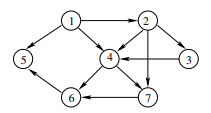
\includegraphics{graph-example}%
\end{minipage}~~%
\begin{minipage}[b]{0.45\columnwidth}%
\texttt{1 2 4 5}

\texttt{2 3 4 7}

\texttt{3 4}

\texttt{4 6 7}

\texttt{5}

\texttt{6 5}

\texttt{7 6}%
\end{minipage}\smallskip{}

\begin{itemize}
\item We assume that the graph we are dealing with is sparse and unweighted.
Then, \textbf{adjacency lists} will be a natural choice to store the
connection between two vertices. The class \texttt{Graph} is used
to store the graph and implements the necessary operations such as
\texttt{buildGraph}. Furthermore, a \texttt{Vertex} class can be implemented
to store the basic information about a graph vertex such as a label
which in our case is an integer. 
\item The vertices are not necessarily numbered consecutively, making a
\textbf{hash table} a logical choice data structure for storing vertices
with labels as keys
\item You may assume that the graph is fully specified by the input stream
and will not be changed after building the graph. Note: The last row
of the input file may or may not be an empty line. Hence, while parsing
consider this case and ignore this last empty line if it exists.
\item \texttt{displayGraph()} will print out each vertex and its adjacency
list. For example, consider the graph $G$ and its corresponding adjacency
linked lists for an input sample graph (\texttt{input.data}). Test
your program by reading a graph from an input file and use the function
\texttt{displayGraph()} to display the generated graph in text format,
see the output below.

\begin{minipage}[t]{0.45\columnwidth}%
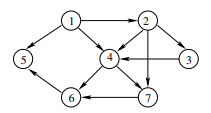
\includegraphics{graph-example}%
\end{minipage}~%
\begin{minipage}[b]{0.4\columnwidth}%
$1:2\,\,\,4\,\,\,5\,$

$2:3\,\,\,4\,\,\,7\,$

$3:4\,$

$4:6\,\,\,7\,$

$5:$

$6:5$

$7:6$%
\end{minipage}

Gradescope should accept the display of vertices in any order (the
column before ``:'') and the adjacent vertices of a vertex in any
order (the list of vertices after ``:'' of a vertex). For example,
valid outputs of \texttt{input.data} are

~%
\begin{minipage}[b]{0.4\columnwidth}%
$7:6$

$6:5$

$5:$

$1:2\,\,\,4\,\,\,5\,$

$2:3\,\,\,4\,\,\,7\,$

$3:4\,$

$4:6\,\,\,7\,$%
\end{minipage}
\item You can compile your code using this command line:

\texttt{\textbf{make}}

And you can run your program by executing:

\texttt{\textbf{./main input.data}}

\smallskip{}

\end{itemize}

\subsection*{Part 2 (60 points)}
\begin{itemize}
\item The formal definition of the topological sort:

\noindent\fbox{\begin{minipage}[t]{1\columnwidth - 2\fboxsep - 2\fboxrule}%
Let G be a DAG with $n$ vertices. A \textbf{topological ordering}
of G is the ordering $v_{1},v_{2},\dots,v_{n}$ of the vertices of
G such that for every edge $(v_{i},v_{j})$ of G we have $i<j$. %
\end{minipage}}
\item The illustration of the definition of the topological sort ordering
gives a sequence of vertices:

\begin{minipage}[t]{0.45\columnwidth}%
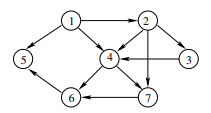
\includegraphics{graph-example}%
\end{minipage}~~%
\begin{minipage}[b]{0.4\columnwidth}%
\texttt{1 2 3 4 7 6 5 }%
\end{minipage}\smallskip{}

The topological sort ordering places vertices of the graph along the
horizontal line with the following property: if there is an edge from
the vertex $v_{i}$ to the vertex $v_{j}$ then the vertex $v_{i}$
precedes $v_{j}$ in the topological ordering.
\item Topological sort algorithm: 
\begin{enumerate}
\item The input is a DAG
\begin{enumerate}
\item Algorithm -- see the textbook, Fig. 9.7, p. 385 or \textbf{Algorithms}
section below. 
\begin{itemize}
\item You can use \texttt{topNum} (\texttt{top\_num}) as in Fig. 9.7 (Image
is provided in \textbf{Algorithms} section as well), and then traverse
the graph to initialize the topological sort ordering vector. \texttt{top\_num}
keeps track of the order of vertices in topological sort. 
\end{itemize}
\item The output of the program should be a vector of vertices (or their
labels) set in topological sort order. 
\begin{itemize}
\item You need to print the topological sort ordering vector by printing
the labels of vertices.
\end{itemize}
\end{enumerate}
In this part you should implement the following functions:
\begin{itemize}
\item \texttt{\small{}bool topological\_sort() }~\\
\texttt{\small{}//performs the topological sort which returns true}~\\
\texttt{\small{}// if a topological ordering is found, }~\\
\texttt{\small{}// otherwise returns false.}{\small\par}
\item \texttt{\small{}void compute\_indegree() }~\\
\texttt{\small{}//assigns the indegree, the number of inbound edges,
}~\\
\texttt{\small{}// for each vertex }{\small\par}
\end{itemize}
\end{enumerate}
\end{itemize}
\smallskip{}


\subsection*{Requirements}
\begin{itemize}
\item Submit only the file \texttt{graph.h} to Gradescope.
\item \textbf{Testing:} test your program for correctness using the cases
below:

\textbf{Case 1}: Use the example (\texttt{input.data}) provided in
the description of the problem.

\textbf{Case 2}: Samantha plans her course schedule. She is interested
in the following eight courses: CSCE121, CSCE222, CSCE221, CSCE312,
CSCE314, CSCE313, CSCE315, and CSCE411. The course prerequisites are:\smallskip{}

\begin{tabular}{cccc}
\textbf{course} & \textbf{\#} & \multicolumn{2}{c}{\textbf{prerequisites}}\tabularnewline
\hline 
CSCE121: & 1 & (none) & \tabularnewline
CSCE222: & 2 & (none) & \tabularnewline
CSCE221: & 3 & CSCE121 & CSCE222\tabularnewline
CSCE312: & 4 & CSCE221 & \tabularnewline
CSCE314: & 5 & CSCE221 & \tabularnewline
CSCE313: & 6 & CSCE221 & \tabularnewline
CSCE315: & 7 & CSCE312 & CSCE314\tabularnewline
CSCE411: & 8 & CSCE222 & CSCE221\tabularnewline
\end{tabular}\smallskip{}

This will find a sequence of courses that allows Samantha to satisfy
all the prerequisites. Assume that she can only take one class at
a time. The input file for this case is provided in \texttt{input2.data}.
Note: the table above contains courses and their prerequisites. The
\texttt{input2.data} file contains the set of vertices and their corresponding
adjacent vertices.

\textbf{Case 3}: Create a directed graph with cycles and test your
program. There is one such a file provided (\texttt{input-cycle.data}).
\item \textbf{Algorithms:}
\begin{itemize}
\item Pseudocode for topological sort (topsort) from the textbook

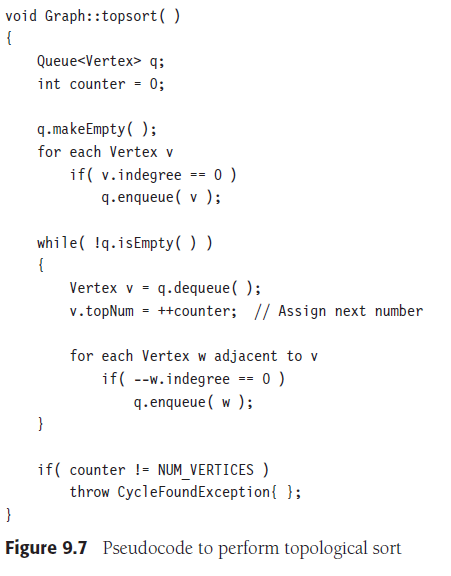
\includegraphics[scale=0.6]{topological_sort}
\item Pseudocode for calculating in-degree from the textbook

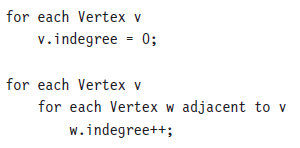
\includegraphics[scale=0.6]{indegree}
\end{itemize}
\item \textbf{Using the C++ Standard Library:}

There are several C++ standard library containers you can use:
\begin{itemize}
\item \texttt{std::unordered\_set}
\item \texttt{std::unordered\_map}
\item \texttt{std::set}
\item \texttt{std::map}
\end{itemize}
The former two use a hash table, the latter two use red-black trees.
The set elements are immutable whereas map elements are mutable. The
other key difference is that the unordered data structures require
the elements to have an ordering defined via \texttt{operator<}. This
allows the in-order traversal of vertices based on this ordering.
This would have been great for \texttt{print\_top\_sort()}, however,
as the topological ordering is not known at insertion time, this cannot
be used for ordering; \texttt{std::unordered\_map} is the \emph{preferable}
data structure. 

To aid in working with this data structure, the following code is
provided:

\begin{lstlisting}[language={C++},basicstyle={\small\ttfamily},showstringspaces=false,tabsize=4]
//create the unordered_map object 
//the two template types are for key and value type 
unordered_map<T, Vertex<T>> node_set;
\end{lstlisting}

\begin{lstlisting}[language={C++},basicstyle={\small\ttfamily},showstringspaces=false,tabsize=4]
//create and insert a new object with key token 
//  if a key in the table with this item exists, 
//  the new object is not inserted 
//returns a pair<unordered_map<T, Vertex<T>>::iterator, bool> 
//  where iterator is a reference to the object in the hash table,
//  bool is true if this is the first time insert, false otherwise 
auto pair = node_set.insert(make_pair(label, Vertex<T>(label)));

bool newItem = pair.second; //true if this is the first item with the given key 

unordered_map<T, Vertex<T>>::iterator iter = pair.first; 

//the iterator can be dereferenced to get the object back 
Vertex<T> v = *iter; //create a copy of the v object 
Vertex<T>& v = *iter; //create a reference to v in the map   

//WARNING: references are only valid until the next insert is made  
//  - they should never be stored in variables
//  - pointers to them should never be made


//Working with STL data structures require considering 
// when references and copies are used.
//The trivial solution is here: 
Vertex<T> v = node_set.at(label); //copy assignment for v . 
v.top_num = 0; //or other changes to v 
node_set.at(label) = v;
\end{lstlisting}

\begin{lstlisting}[language={C++},basicstyle={\small\ttfamily},showstringspaces=false,tabsize=4]

//Alternatively, using references can save some copies 
//top_num is 0 by default 
cout << node_set.at(label).top_num << endl;   // outputs 0
Vertex<T>& vRef = node_set.at(label);       // by reference 
vRef.top_num += 1;  //incrementing the object in the map 
cout << node_set.at(label).top_num << endl;   // outputs 1 
Vertex<T> vCopy = node_set.at(label);  //copy assignment 
vCopy.top_num += 1;             // increments the copy 
cout << node_set.at(label).top_num << endl; // outputs 1 again 
node_set.at(label).top_num += 1; //incrementing the object in the map  
cout << node_set.at(label).top_num << endl;   // outputs 2
\end{lstlisting}

\begin{lstlisting}[language={C++},basicstyle={\small\ttfamily},showstringspaces=false,tabsize=4]
//much of the same applies to iterating the map object 
//elements by reference, updates within the map 
for(auto& v: node_set){ 
  v.second.indegree = 0;
} 
//elements by copy, no updates to the item in the map 
for(auto v: node_set){
  v.second.indegree = 0;
} 
//in both the cases auto is pair<T,Vertex<T>> type object 
//in case this is a new syntax for you:
// these for loops are iterating over all objects in the map
\end{lstlisting}

(\emph{Optional}) Another data structure you may be using for the
first time is \texttt{std::priority\_queue}, implemented via a binary
heap. It takes one or three template parameters: \texttt{<Type, ContainerType,
Functor>}. The priority queue orders by maximizing, meaning that the
greatest priority element is returned first. The stored type or the
functor should implement the \texttt{operator<()}. The Container type
is unimportant, \texttt{std::vector<Vertex<T>\textcompwordmark >}
can be used. The code for declaring a functor class is show below.
Recall that the implementation of topological ordering likely assigns
the first ordered elements a lower value.

\begin{lstlisting}[language={C++},basicstyle={\small\ttfamily},showstringspaces=false,tabsize=4]
// syntax for a custom comparator
template<class T> 
class VertexCompare {
public:
  bool operator()(Vertex<T> v1, Vertex<T> v2){
    //TODO - implement
	return false;
  }
};
...
priority_queue<Vertex<T>, vector<Vertex<T>>, VertexCompare<T>> pq;
\end{lstlisting}
\end{itemize}

\end{document}
